% !TEX root = sum1.tex
\section{Problem Description}
In this section, we first consider the seat planning problem with social distancing. Then we introduce the dynamic seat assignment problem with social distancing.

% Then we incorporate the social distancing into seat planning.

% give the description of the seat planning problem with social distancing.

% dynamic seat assignment problem, which is suitable for commercial use in cinemas and concerts.


\subsection{Seat Planning Problem with Social Distancing}\label{dynamic_demand}
We consider a set of groups, each of which consists of no more than $M$ people, to be assigned to a set of seats. There are $M$ different group types, with group type $i$ containing $i$ people, where $i \in [M] \coloneqq \{1,2, \ldots, M\}$. (We use $[M] = \{1, \ldots, M\}$ to denote the set of all positive integers that are no larger than $M$.)

These groups can be represented by a demand vector, denoted by $\mathbf{d} = [d_1, \ldots, d_M]_d$. Each element $d_i$, where $i \in [M]$, indicates the number of group type $i$. For illustration, we consider a layout consisting of $N$ rows, each containing $S_j$ seats, where $j \in [N]$.

In accordance with epidemic prevention requirements, customers from the same group are allowed to sit together, while different groups must maintain social distancing. Let $s$ denote the social distancing, which can be one seat or more seats.

Specifically, each group must leave empty seat(s) to maintain social distancing from adjacent groups. Additionally, different rows do not affect each other, meaning that a person from one group can sit directly behind a person from another group.

% We consider the social distancing of one empty seat throughout the rest of this paper, which is more practical and reasonable in the seat planning. However, our methods are still applicable to the social distancing of two or more seats.


To achieve the social distancing requirements in the seat planning process, we add $s$ to the original size of each group to create the new size of the group. Let $n_i = i + s$ denote the new size of group type $i$ for each $i \in [M]$. Construct new seat layout by adding $s$ to each row, i.e., let $L_j = S_j + s$ denote the length of row $j$ for each $j \in [N]$, where $S_j$ represents the number of seats in row $j$.


Then we can illustrate the seat planning for one row below. 

\begin{figure}[ht]
    \centering
    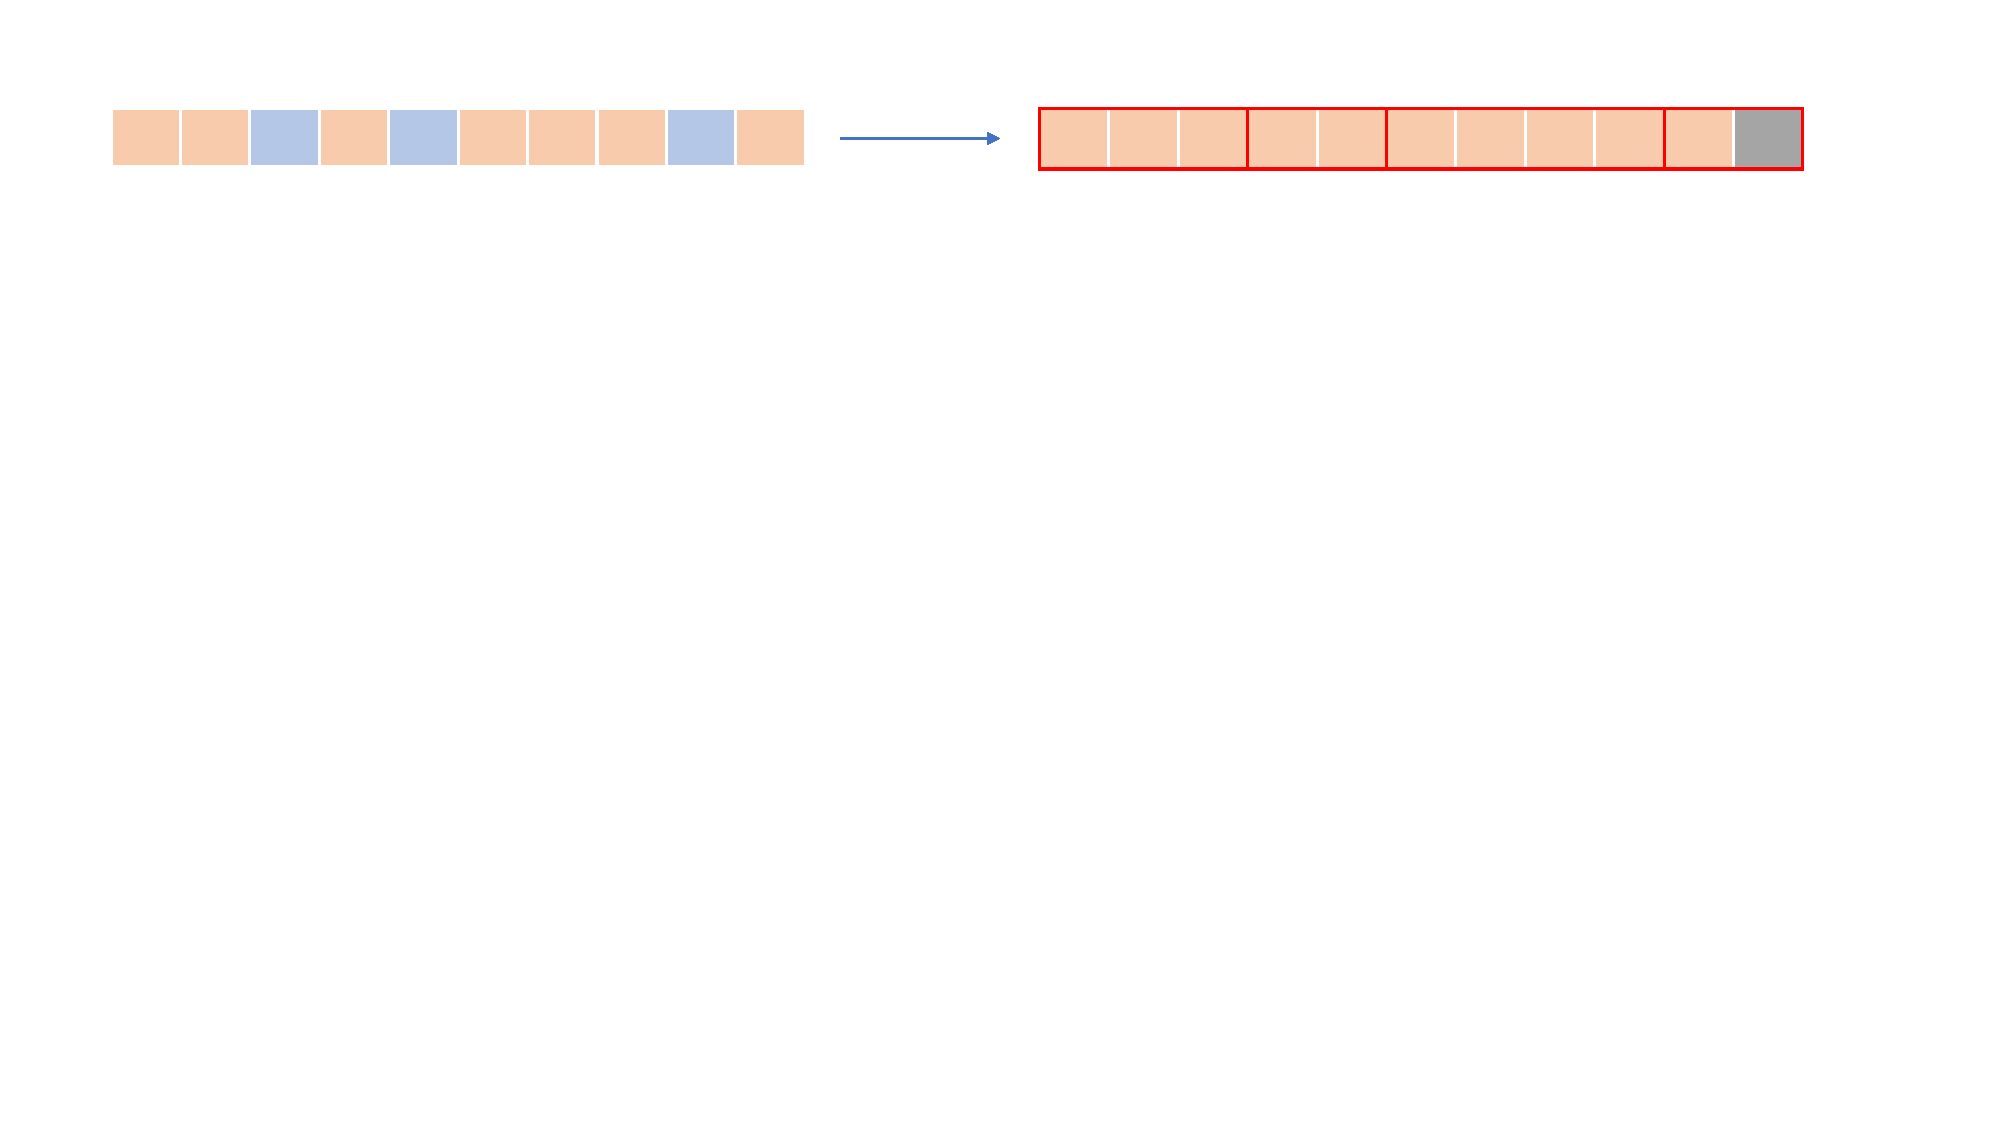
\includegraphics[width = 0.8\textwidth]{./Figures/dummy_seat.pdf}
    \caption{Problem Conversion}
\end{figure}

The social distancing here is one seat. On the left side of the diagram, the blue squares represent the empty seats required for social distancing, while the orange squares represent the seats occupied by groups. On the right side, we have added one dummy seat at the end of each row. The orange squares surrounded by the red line represent the seats taken by groups in this row, which includes two groups of 1, one group of 2, and one group of 3.

By incorporating the additional seat and designating certain seats for social distancing, we can integrate social distancing measures into the seat planning problem.


Now, we analyse the effect of introducing social distancing for each row. At first, we consider the types of pattern, which refers to the seat planning for each row. For each pattern $k$, we use $\alpha_k, \beta_k$ to indicate the number of groups and the left seats, respectively. Denote by $l(k) = \alpha_k + \beta_k -1$ the loss for pattern $k$. The loss represents the number of people lost compared to the situation without social distancing.

Let $I_1$ be the set of patterns with the minimal loss. Then we call the patterns from $I_1$ are largest. Similarly, the patterns from $I_2$ are the second largest, so forth and so on. The patterns with zero left seat are called full patterns. Suppose there are $n$ groups in a row, we use a descending form $P_{k} = (t_1, t_2, \ldots, t_n)$ to denote pattern $k$, where $t_h$ is the new group size, $h \in [n]$. 

% Let $P_{k}$ denote the set of group sizes for pattern $k$. We use $t \in P_{k}$ to denote a group with size of $t$ can be put into the pattern. 

\begin{example}
  Suppose the social distancing is one seat, then the new sizes of groups are $2, 3, 4, 5$, respectively. The length of one row is $L = 21$ and the demand is $[10, 12, 9, 8]_d$. Then these patterns, $(5, 5, 5, 5, 1), (5, 4, 4, 4, 4),(5, 5, 5, 3, 3)$, belong to $I_1$. For pattern 1, $(5, 5, 5, 5, 1)$, $P_{1} = \{5\}$, thus a group with a size smaller than 5 cannot be put in this pattern.
\end{example}

% To represent a pattern with a fixed length of form, we can use a $(M+1)-$dimensional vector with $M$ group types. The aggregated form can be expressed as $[n_0, n_1, \ldots, n_M]$, where $n_i$ is the number of $i$-th group type, $i \in [M]$. $n_0$ is the number of left seat, its value can only be $0, 1$ because two or more left seats will be assigned to groups. Thus the pattern, $[1, 0, 0, 0, 4]$, is not full because there is one left seat.

For ease of brevity, we suppose $u$ is the new size of the largest group allowed, then $u = M+s$.
We can use the following greedy way to generate the largest pattern. Select the maximal group size, $u$, as many as possible and the left space is assigned to the group with the corresponding size. Let $L = u\cdot q + r, 0 \leq r < u$, where $q$ is the number of times $u$ selected. When $r>0$, there are $d[0][u-r][q+1]$ largest patterns with the same loss of $q$. When $r =0$, there is only one possible largest pattern.

% all possible seats can be assigned are the consecutive integers from 2 to $u$. 

Use dynamic programming to solve. $d[k][i][j]$ indicates the number of assignment of using $i$ capacity to allocate $j$ units, $k$ is the number of capacity allocated on the last unit. In our case, $u-r$ is the capacity need to be allocated, $q+1$ is the number of units which corresponds to the groups. Notice that we only consider the number of combinations, so we fix the allocation in ascending order, which means the allocation in current unit should be no less than the last unit.  

The number of largest patterns equals the number of different schemes that allocate $u-r$ on $q+1$ units,i.e., $d[0][u-r][q+1]$.

The recurrence relation is $d[k][i][j] = \sum_{t=k}^{i-k} d[t][i-k][j-1]$. 
When $i < k$, $d[k][i][j] =0$; when $i \geq k$, $d[k][i][1] =1$.

\begin{lem}
When given the length of row, $L$, and the new size of the largest group allowed, $u$. Let $L = u\cdot q + r$, then the loss of the largest pattern is $q - f(r)$, where $f(r) =1$ if $r=0$; $f(r) =0$ if $r \neq 0$.
\end{lem}

\begin{lem}
The seat assignment made up of the largest patterns is optimal.
\end{lem}

This lemma holds because we cannot find a better solution occupying more seats. When the demand can meet that the largest patterns can be generated in all rows, an optimal seat assignment can be obtained.

\begin{prop}
For a seat layout, $\{S_1, S_2, \ldots, S_{N}\}$, the total loss is $\sum_{j} (\lfloor \frac{S_j+1}{u}  \rfloor - f((S_j +1)\mod u))$. The maximal number of people assigned is $\sum_{j} (S_j - \lfloor \frac{S_j+1}{u} \rfloor + f((S_j +1)\mod u))$.
\end{prop}

\subsection{Dynamic Seat Assignment with Social Distancing}
% In this section we present the model that generates seat planning under deterministic demands.

% Let the $i-$th group type contain $i$ people. 
% $(d_1, d_2, d_3, d_4) = (3,5,7,6)$

% But our model and formulation allow for a more general layout of the seats. 
Now consider the scenario where groups arrive dynamically, the decision-maker must determine whether to accept or reject each group and assign them to empty seats while ensuring that the social distancing constraint is met. Once the seats are confirmed and assigned to a group, they cannot be changed.

We use a vector $\mathbf{L}= (L^{r}_1, L^{r}_2, \ldots, L^{r}_{N})$ to record the remaining capacity of rows, where $L^{r}_{j}$ represents the number of remaining seats in row $j$. Let $V_{t}(\mathbf{L})$ denote the maximal expected value to go at period $t$ with capacity of rows. Let $\mathbf{w} = (n_1, \ldots, n_{M})$ be the number of seats occupied by each group type. There are $T$ periods and the arrival probability of the group type $i$ in each period is $p_i$. In every period, the group can decide which row to sit.

The dynamic programming formulation for this problem is
$$V_{t}(\mathbf{L}) = E_{i} \left[ \max_{k \in N: L_k \geq i + s} \{ {[V_{t-1}(\mathbf{L}- (\mathbf{w} \circ \mathbf{e}_{i})U_{k})+ i]}, {V_{t-1}(\mathbf{L})}\} \right], \mathbf{L} \geq \mathbf{0}, V_{T+1}(\mathbf{L}) = 0,$$

where $\circ$ in $\mathbf{w} \circ \mathbf{e}_{i}$ is the element-wise product, $\mathbf{e}_{i}$ is the unit vector whose i-th element is 1, $U_k$ is a matrix of $m$ by $n$ with all elements in column $k$ being 1.  Initially, we have $\mathbf{L}_{T} = (L_1, L_2, \ldots, L_{N})$. 

% use ei to denote a row vector of 0’s, but with 1 at the ith entry

As we can observe, the dynamic programming algorithm has to make a decision on which row to assign group type $i$. This leads to the curse of dimensionality due to the numerous seat planning combinations. To avoid this complexity, we propose an approach that directly targets the final seat planning and then formulate a policy for assigning groups. To obtain the final seat planning firstly, we develop the scenario-based stochastic programming.

% The number of all seats in each row is called the length of the row.

% when the capacity allows accepting the groups from large to small as many as possible will give an optimal solution.


% Why is it easy to solve this IP?

% If the ratio is the same for the groups, IP will use more branches to obtain an optimal solution.

% $[24,28,8,9]$ 10 rows.
% Total loss: 60; loss of the largest pattern: 5.


% Specifically, we define the concept of target seating plans deemed satisfactory. In making the dynamic seating plan, we will try to maintain the possibility of achieving one of the target seating plans as much as possible.
